\documentclass[10pt]{article}
\usepackage[utf8]{inputenc}
\usepackage[english]{babel}
\usepackage[font=small,labelfont=bf]{caption}
\usepackage{geometry}
\usepackage[sort&compress, numbers, super]{natbib}
\usepackage{pxfonts}
\usepackage{graphicx}
\usepackage{setspace}
\usepackage{hyperref}
\usepackage{lineno}

\newcommand{\argmax}{\mathop{\mathrm{argmax}}\limits}

%\newcommand{\demo}{S1}

\doublespacing
\linenumbers

\title{Carryover clustering effects in free recall reveal how prior experiences influence memory for new experiences}
\author{Jeremy R. Manning\textsuperscript{1, *}, Andrew C. Heusser\textsuperscript{1, 2}, Kirsten Ziman\textsuperscript{1, 3},\\Emily Whitaker\textsuperscript{1}, and Paxton C. Fitzpatrick\textsuperscript{1}\\\textsuperscript{1}Dartmouth College\\\textsuperscript{2}Akili Interactive\\\textsuperscript{3}Princeton University\\\textsuperscript{*}Corresponding author: jeremy.r.manning@dartmouth.edu}

\date{}

\begin{document}
\maketitle

\begin{abstract}
Insert abstract here
\end{abstract}


\section*{Main text}
Insert text here (Figs.~\ref{fig:demo}, \demo).

\begin{figure}[tp]
\centering
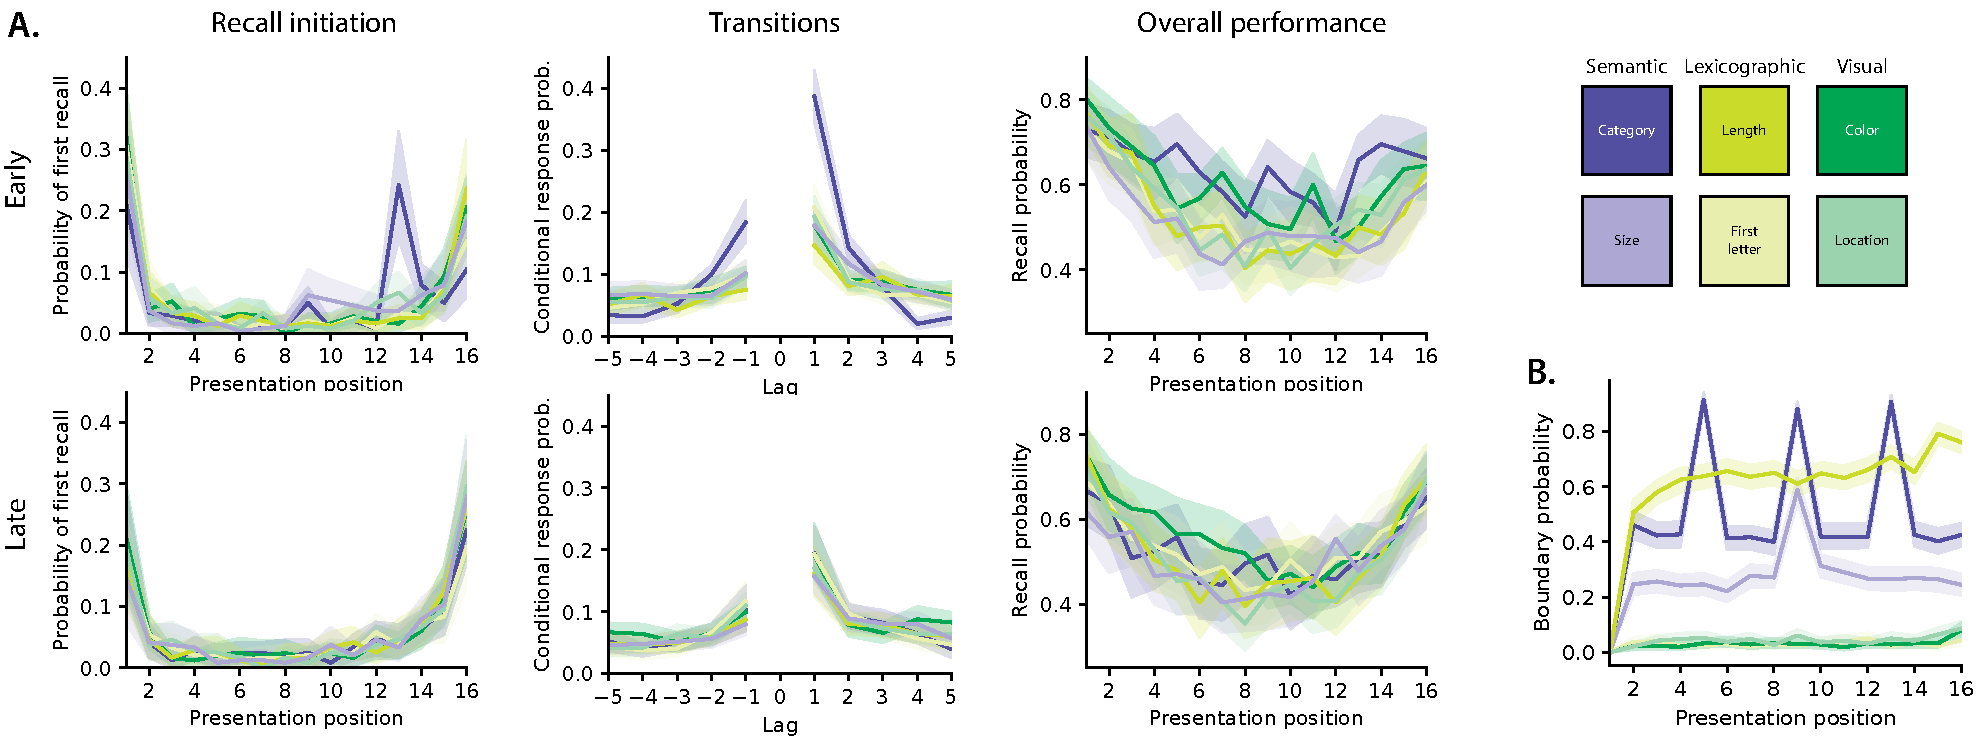
\includegraphics[width=\textwidth]{figures/recall_dynamics}
\caption{\textbf{Recall dynamics in free recall.}}
\label{fig:recall-dynamics}
\end{figure}

\bibliographystyle{apa}
\bibliography{cdl}
\end{document}
